\documentclass[11pt,a4paper]{article}
\usepackage[T1]{fontenc}
\usepackage[margin=2.3cm]{geometry}
\usepackage{amsmath,amssymb}
\usepackage{graphicx}
\usepackage[dvipsnames]{xcolor}
\usepackage{enumitem}
\usepackage[colorlinks=true,linkcolor=blue,urlcolor=blue]{hyperref}
\setlength{\parskip}{0.6em}
\setlength{\parindent}{0pt}
\begin{document}

\begin{center}{\LARGE\bfseries openinduction}\\[0.4em]{\large Spin a coil, step a voltage down: how generators and transformers work, in three sessions.}\\[0.2em]\small PAN IIT OSS explainer \textbullet{} secondary school to diploma / undergraduate (levels 3-5)\end{center}

\section*{Why this exists}
Every power station, bicycle dynamo and phone charger runs on one law: a changing magnetic flux through a coil makes a voltage. This explainer follows that law from a magnet and a coil to a spinning generator and a transformer, with simple mathematics and a few lines of Python.

\section*{The end goal}
Explain how a transformer and a generator work from Faraday's law. The end goal is to explain how a transformer and a generator work from Faraday's law: why a rotating coil gives an alternating voltage, how a transformer steps it up or down, and where the energy and the losses go. All models are simplified, low-voltage teaching models and are not design tools.

\section*{How the three sessions build up}
\begin{enumerate}[nosep]
\item \textbf{Session 1: A changing flux makes a voltage} (Level 1, conceptual interactive model, 60 min).
\item \textbf{Session 2: Faraday's law, the sine wave and the transformer} (Level 2, mathematical engineering model, 75 min).
\item \textbf{Session 3: A loaded generator, transformer losses and saturation} (Level 3, simulation and validation, 90 min).
\end{enumerate}

\section{Session 1: A changing flux makes a voltage}

\subsection*{A. Real-world problem}
A bicycle dynamo has no battery, yet it lights a lamp when you pedal. Inside there is only a magnet and a coil of wire, and nothing touches. The same trick runs every power station: something turns, and a voltage appears. Where does that voltage come from, and what makes it bigger or smaller? This is a low-voltage educational model: we use small numbers and never work with mains electricity.

\subsection*{B. Concept and theory}
Magnetic flux (symbol Phi) measures how much magnetic field passes through a coil: a stronger field, or a bigger coil facing the field, means more flux. Faraday found that a coil produces a voltage (called an EMF, electromotive force) only while the flux through it is changing. The size of the voltage is the number of turns times the rate of change of the flux. A magnet at rest, however strong, makes no voltage. Push the magnet in and the voltage has one sign; pull it out and the sign reverses: this is Lenz's law, the induced voltage opposes the change that caused it. If the coil spins in a field, the flux rises and falls in every turn, so the voltage swings positive and negative: alternating current (AC). The peak voltage is N B A 2 pi f.

\begin{itemize}[nosep]
\item emf: induced voltage (electromotive force) (V)
\item N: number of turns of the coil (no unit)
\item Phi: magnetic flux through one turn (Wb (weber))
\item delta Phi / delta t: change of flux divided by the time taken (Wb/s)
\item B: magnetic field strength (T (tesla))
\item A: area of the coil (m\textasciicircum{}2)
\item f: turns per second, the frequency (Hz)
\end{itemize}

\begin{equation*}
\mathcal{E}_{\mathrm{avg}} = N\,\frac{\Delta\Phi}{\Delta t}
\end{equation*}

\begin{equation*}
\Phi = B A\cos\theta
\end{equation*}

\begin{equation*}
\mathcal{E}_{\mathrm{peak}} = N B A\,2\pi f
\end{equation*}

\begin{center}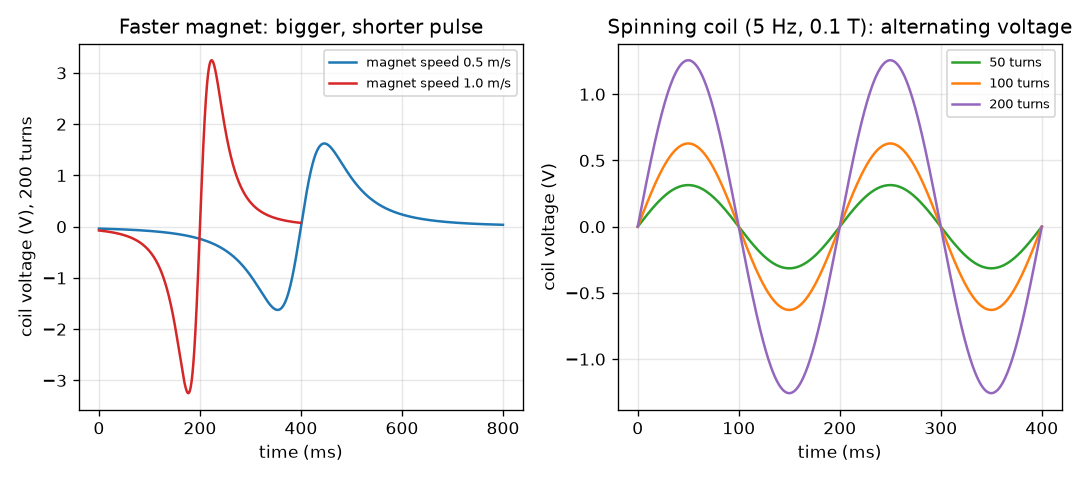
\includegraphics[width=0.85\linewidth]{figures/s01_magnet_and_coil.png}\\\small Left: a magnet pushed through a 200 turn coil at two speeds. Right: a spinning coil at 5 Hz makes alternating voltage that grows with the turns.\end{center}

\subsection*{E. Worked example}
(a) A magnet pushed into a 200 turn coil changes the flux through it by 0.5 mWb in 0.05 s. What is the average voltage, and what if the push takes 0.025 s? (b) What is the peak voltage of a coil with 100 turns, area 0.002 m\textasciicircum{}2, spun at 5 Hz in a 0.1 T field?
\begin{enumerate}[nosep]
\item (a) Convert 0.5 mWb = 0.0005 Wb. Voltage = N x delta Phi / delta t = 200 x 0.0005 / 0.05 = 2.0 V.
\item Twice as fast: 200 x 0.0005 / 0.025 = 4.0 V. Twice the speed, twice the voltage.
\item (b) Peak = N B A 2 pi f = 100 x 0.1 x 0.002 x 2 x 3.1416 x 5.
\item 100 x 0.1 x 0.002 = 0.02, and 2 pi x 5 = 31.416, so peak = 0.02 x 31.416 = 0.628 V.
\end{enumerate}
\textbf{Answer.} (a) 2 V, and 4 V when the push is twice as fast. (b) The peak is 0.628 V.

\subsection*{F. Questions}
\begin{enumerate}[nosep]
\item \textbf{Conceptual.} Why does a strong magnet resting inside a coil make no voltage? And where does the electrical energy come from when you push the magnet in?
\item \textbf{Numerical.} A coil of 500 turns sees the flux through it grow from 0 to 0.2 mWb in 0.02 s. What is the average voltage? Check that the answer is sensible.
\item \textbf{Graph and simulation interpretation.} In the left figure the magnet speed is doubled. What happens to (i) the peak voltage, (ii) how long the pulse lasts, (iii) the area of one pulse?
\item \textbf{Design and optimisation challenge.} Design: you want a spinning coil with a peak voltage of 3 V. You have N = 100 turns, A = 0.002 m\textasciicircum{}2 and a 0.1 T magnet. What frequency do you need? If your hand can only turn the coil at 5 Hz, how many turns would you need instead? What is the trade-off?
\end{enumerate}

\section{Session 2: Faraday's law, the sine wave and the transformer}

\subsection*{A. Real-world problem}
You want a hand-crank torch with no battery: how many turns of wire, how strong a magnet and how fast a crank give a few volts? And your phone charger has to turn the 230 V of the wall socket into a safe low voltage: how many turns does each side need, and how much current flows? Both questions are answered by one law. This is an ideal, low-voltage teaching model: the mains numbers below are for calculation only and you must never experiment with mains electricity.

\subsection*{B. Concept and theory}
Flux through a flat coil of area A in a uniform field B, where theta is the angle between the field and the coil's normal, is Phi = B A cos(theta). Faraday's law says EMF = -N dPhi/dt: the voltage is minus the number of turns times the rate of change of flux (the minus sign is Lenz's law). If the coil turns at constant angular speed w = 2 pi f, then theta = w t, Phi = B A cos(w t) and differentiating gives EMF = N B A w sin(w t), with peak N B A w. Notice the EMF is zero when the flux is largest and largest when the flux is zero (the flux changes fastest as it passes through zero). The RMS value of a sine, the DC value that heats a resistor equally, is peak / sqrt(2). Mains is 50 Hz in many countries: a period of 20 ms and 230 V RMS means a peak of 325 V. An ideal transformer has two coils of N1 and N2 turns on one iron core. The same changing flux threads both coils, so each turn gets the same voltage and V2/V1 = N2/N1. If nothing is wasted, power in equals power out, V1 I1 = V2 I2, so I2/I1 = N1/N2: stepping the voltage down steps the current up. It works only with changing flux: DC makes no flux change and no secondary voltage.

\begin{itemize}[nosep]
\item Phi: flux through one turn (Wb)
\item B: magnetic field (T)
\item A: coil area (m\textasciicircum{}2)
\item theta: angle between field and coil normal (rad)
\item N: number of turns (no unit)
\item w: angular speed, 2 pi f (rad/s)
\item f: frequency (Hz)
\item EMF: induced voltage (V)
\item V1, V2: primary and secondary RMS voltage (V)
\item I1, I2: primary and secondary RMS current (A)
\item N1, N2: primary and secondary turns (no unit)
\end{itemize}

\begin{equation*}
\Phi(t) = B A\cos(\omega t)
\end{equation*}

\begin{equation*}
\mathcal{E} = -N\frac{d\Phi}{dt} = N B A\,\omega\sin(\omega t),\qquad \omega = 2\pi f
\end{equation*}

\begin{equation*}
E_{\mathrm{rms}} = \frac{E_{\mathrm{peak}}}{\sqrt{2}},\qquad T = \frac{1}{f}
\end{equation*}

\begin{equation*}
\frac{V_2}{V_1} = \frac{N_2}{N_1},\qquad \frac{I_2}{I_1} = \frac{N_1}{N_2},\qquad V_1 I_1 = V_2 I_2
\end{equation*}

\begin{center}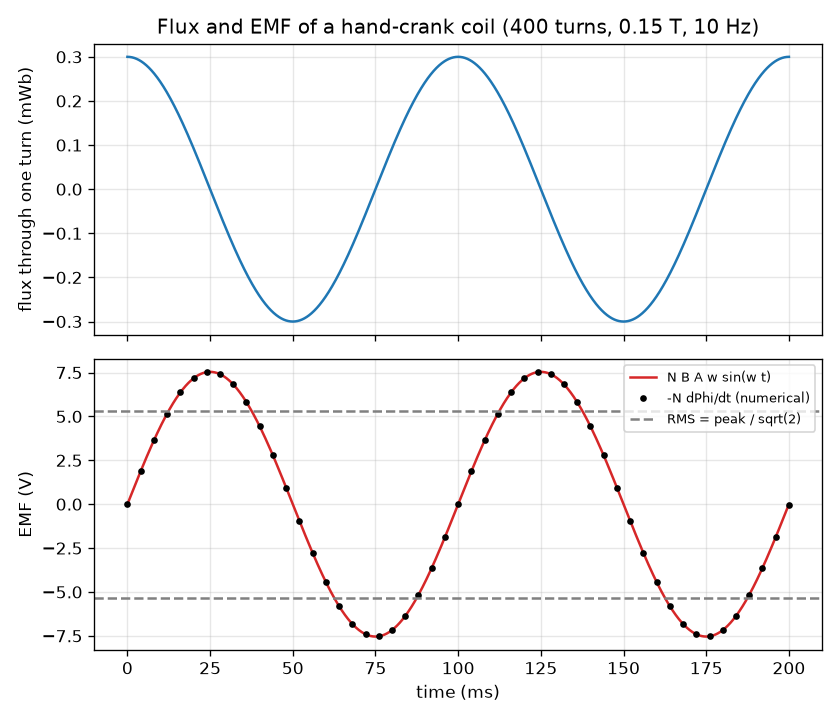
\includegraphics[width=0.85\linewidth]{figures/s02_flux_and_emf.png}\\\small Flux and EMF of the hand-crank coil: the EMF is a quarter period out of step with the flux and the numerical derivative matches the formula.\end{center}

\subsection*{E. Worked example}
(a) A hand crank turns a coil of 400 turns, area 0.002 m\textasciicircum{}2, in a 0.15 T field at 10 Hz. Find the peak and RMS EMF. (b) Design a transformer to supply a 24 W load at 12 V from 230 V: find the turns ratio, the primary turns if the secondary has 24 turns, and both currents.
\begin{enumerate}[nosep]
\item (a) w = 2 pi x 10 = 62.83 rad/s. Peak = N B A w = 400 x 0.15 x 0.002 x 62.83 = 7.54 V.
\item RMS = 7.54 / sqrt(2) = 5.33 V. The period is 1/10 = 100 ms.
\item (b) Turns ratio N1/N2 = 230 / 12 = 19.17. With N2 = 24, N1 = 24 x 19.17 = 460 turns.
\item Secondary current I2 = P / V2 = 24 / 12 = 2.0 A.
\item Primary current I1 = P / V1 = 24 / 230 = 0.104 A. Check: I2 x N2/N1 = 2.0 / 19.17 = 0.104 A, and V1 I1 = 24 W = V2 I2.
\end{enumerate}
\textbf{Answer.} (a) peak 7.54 V, RMS 5.33 V. (b) ratio 19.17 : 1, N1 = 460 turns for N2 = 24, I2 = 2.0 A, I1 = 0.104 A.

\subsection*{F. Questions}
\begin{enumerate}[nosep]
\item \textbf{Conceptual.} Why does a transformer work on AC but not on DC? What happens to the current in the primary when you connect a transformer to DC?
\item \textbf{Numerical.} A coil of 200 turns, area 0.005 m\textasciicircum{}2, turns at 25 Hz (1500 rpm) in a 0.2 T field. Find the peak and RMS EMF. Check the units.
\item \textbf{Graph and simulation interpretation.} In the flux and EMF graph of the hand-crank coil (10 Hz), at which times is the EMF zero and at which times is it largest? What is the flux at those moments?
\item \textbf{Design and optimisation challenge.} Design: a small device needs 5 V at 10 W from 230 V. Choose N2 = 20 turns. Find N1, I2 and I1. Why do small transformers not use very few turns?
\end{enumerate}

\section{Session 3: A loaded generator, transformer losses and saturation}

\subsection*{A. Real-world problem}
A bicycle dynamo lights a 3 W lamp, but its coil has resistance and inductance, so the lamp never sees the full EMF. A transformer is warm after a while because its wire has resistance and its iron wastes energy. And if you push too much flux into the iron, the output is no longer a clean sine wave. Can we simulate these effects, check that no energy is created or lost, and use the model to choose a design? All numbers are illustrative low-voltage teaching values, not measurements of a real machine, and nothing here is a design method for real generators or transformers.

\subsection*{B. Concept and theory}
Generator: the coil EMF e = N B A w sin(w t) drives the armature resistance Ra, the armature inductance L and the load RL in series, so L di/dt = e - (Ra + RL) i. We integrate this with the Runge-Kutta 4th-order method (RK4) and also integrate the energies. The exact steady state is a sine of peak Em / Z where the impedance Z = sqrt((Ra + RL)\textasciicircum{}2 + (w L)\textasciicircum{}2); the current lags the EMF by arctan(w L / (Ra + RL)). The magnetic torque on the current-carrying coil is tau = -N B A i sin(w t): its sign is opposite to the rotation when e i is positive. That is Lenz's law, and it means the shaft must supply the mechanical power -tau w = e i. Averaged over whole periods this equals the power in the load plus the heat in the armature resistance. Transformer: the equivalent circuit adds winding resistances (copper loss I\textasciicircum{}2 Req), a leakage reactance and a core-loss resistance Rc across the primary (core loss V1\textasciicircum{}2 / Rc, present even with no load). Efficiency is output power over input power, and voltage regulation is the fractional drop of the secondary voltage from no load to load. Efficiency is highest where the copper loss equals the core loss. Saturation: a real iron core can carry only a limited flux. We model the flux linkage as lambda = lambda\_s tanh(i / i\_s). When the supply pushes more volt-seconds than lambda\_s allows, the current spikes and the output is distorted. The equation d lambda/dt = v - rs i is stiff near saturation, so we use implicit backward Euler with a bisection solve. The tanh model is an illustrative teaching model.

\begin{itemize}[nosep]
\item Ra, L, RL: armature resistance, armature inductance, load resistance (ohm, H, ohm)
\item Em: peak EMF, N B A w (V)
\item Z: impedance of the series circuit (ohm)
\item Irms: RMS current (A)
\item tau: magnetic torque on the coil (N m)
\item Req, Xeq, Rc: equivalent winding resistance, leakage reactance, core-loss resistance (referred to the primary) (ohm)
\item eta: efficiency, P\_out / P\_in (no unit)
\item VR: voltage regulation (no unit)
\item lambda\_s, i\_s: saturation flux linkage and knee current of the core model (Wb-turn, A)
\end{itemize}

\begin{equation*}
L\frac{di}{dt} = E_m\sin(\omega t) - (R_a + R_L)\,i
\end{equation*}

\begin{equation*}
Z = \sqrt{(R_a+R_L)^2 + (\omega L)^2},\qquad I_{\mathrm{rms}} = \frac{E_m}{\sqrt{2}\,Z},\qquad P_{\mathrm{load}} = I_{\mathrm{rms}}^2 R_L
\end{equation*}

\begin{equation*}
\tau = -N B A\, i\sin(\omega t),\qquad P_{\mathrm{mech}} = -\tau\omega = e\,i = P_{\mathrm{load}} + I_{\mathrm{rms}}^2 R_a
\end{equation*}

\begin{equation*}
\eta = \frac{P_{\mathrm{out}}}{P_{\mathrm{out}}+P_{\mathrm{Cu}}+P_{\mathrm{core}}},\qquad \mathrm{VR} = \frac{V_{2,\mathrm{nl}}-V_{2,\mathrm{fl}}}{V_{2,\mathrm{nl}}}
\end{equation*}

\begin{equation*}
\lambda = \lambda_s\tanh\!\left(\frac{i}{i_s}\right),\qquad \frac{d\lambda}{dt} = v - r_s\,i
\end{equation*}

\begin{center}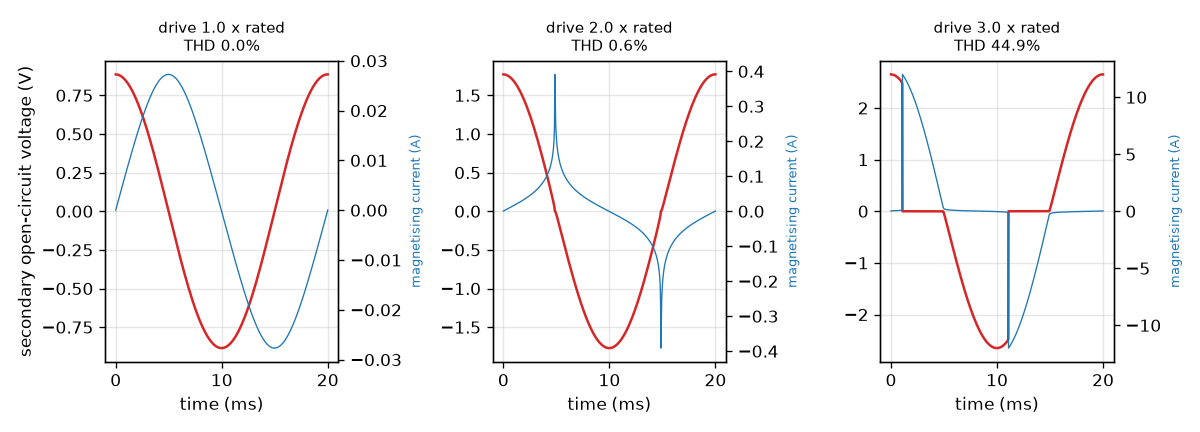
\includegraphics[width=0.85\linewidth]{figures/s03_core_saturation.png}\\\small Saturating core model at 1, 2 and 3 times the rated drive: the secondary voltage distorts once the core saturates.\end{center}

\subsection*{E. Worked example}
(a) A generator with N B A = 0.08 V s runs at 50 Hz with Ra = 2 ohm, L = 30 mH and RL = 10 ohm. Find the peak EMF, Z, RMS current, load power, armature heat and the mechanical power needed. (b) For the 460 : 24 turn transformer with RL = 6 ohm on its secondary and 230 V on the primary, find V2, efficiency and regulation.
\begin{enumerate}[nosep]
\item (a) w = 2 pi x 50 = 314.16 rad/s. Em = 0.08 x 314.16 = 25.13 V. w L = 314.16 x 0.030 = 9.425 ohm.
\item Z = sqrt((2 + 10)\textasciicircum{}2 + 9.425\textasciicircum{}2) = sqrt(144 + 88.83) = 15.26 ohm. Irms = 25.13 / (15.26 x 1.4142) = 1.165 A.
\item Load power = 1.165\textasciicircum{}2 x 10 = 13.56 W. Armature heat = 1.165\textasciicircum{}2 x 2 = 2.71 W. Mechanical power = 13.56 + 2.71 = 16.28 W.
\item The RK4 simulation gives the same load power (13.565 W) and a mechanical power of 16.278 W, with an energy balance residual of about 2e-9 J per 0.08 s. The mean torque is -51.8 mN m: 0.0518 N m x 314.16 rad/s = 16.28 W, so the field opposes the rotation.
\item (b) a = 460 / 24 = 19.17, Req = 30 + 19.17\textasciicircum{}2 x 0.08 = 59.4 ohm, and RL referred to the primary = 19.17\textasciicircum{}2 x 6 = 2204 ohm. Solving the circuit gives V2 = 11.68 V, output 22.75 W, copper loss 0.61 W and core loss 1.51 W (= 230\textasciicircum{}2 / 35000).
\item Efficiency = 22.75 / (22.75 + 0.61 + 1.51) = 91.5 percent. Regulation = (12 - 11.68) / 12 = 2.6 percent.
\end{enumerate}
\textbf{Answer.} (a) Em = 25.13 V, Z = 15.26 ohm, Irms = 1.165 A, load 13.56 W, armature heat 2.71 W, mechanical input 16.28 W. (b) V2 = 11.68 V, efficiency 91.5 percent, regulation 2.6 percent (illustrative values).

\subsection*{F. Questions}
\begin{enumerate}[nosep]
\item \textbf{Conceptual.} A bicycle dynamo is harder to pedal when the lamp is on than when the lamp is off. Explain why using Lenz's law, and say where the energy for the lamp comes from.
\item \textbf{Numerical.} A generator has Em = 20 V peak, Ra = 1 ohm, RL = 9 ohm and negligible inductance. Find the RMS current, the power in the load, the heat in the armature and the mechanical power, and check that they balance.
\item \textbf{Graph and simulation interpretation.} In the transformer efficiency figure, the output power is 0.29 W at a load of 500 ohm. Roughly what is the efficiency there (the curve starts near 16 percent), why is it so low, and why does it fall again beyond the peak at about 33 W?
\item \textbf{Design and optimisation challenge.} Design: for the generator in the worked example (Ra = 2 ohm, L = 30 mH, 50 Hz, Em = 25.13 V), which RL gives the largest load power, and what share of the mechanical power does the armature waste there? What RL would you choose if the armature must waste no more than 10 percent, and what load power do you get?
\end{enumerate}

\section{Real-world mini-project}
\textbf{Design a bicycle dynamo to power a 3 W lamp.} A bicycle lamp is rated 6 V, 3 W, so its resistance is 6\textasciicircum{}2 / 3 = 12 ohm. A small roller of radius 0.01 m runs on the tyre, so the coil turns at w = v / 0.01 rad/s when the bike moves at speed v. The coil has B = 0.3 T, area 4e-4 m\textasciicircum{}2, armature resistance 1.5 ohm and inductance 40 mH. Using \texttt{dynamo\_power} and \texttt{simulate\_generator} from Session 3, find the smallest number of turns (in steps of 10) so that the lamp gets at least 3 W at 15 km/h but no more than 4.5 W at 25 km/h, so the bulb survives a fast downhill ride.

\section{The path ahead}
\begin{enumerate}[nosep]
\item \textbf{Session 4: Three-phase generator.} A generator with three coils feeding three equal loads, with a plot of each phase and of the total power.
\item \textbf{Session 5: AC to DC with a rectifier and capacitor.} A full-wave rectifier model with two diode drops and a capacitor, simulated in time.
\item \textbf{Session 6: A transformer from two coupled coils.} A time-domain model of the primary and secondary currents with winding resistance and a resistive load.
\item \textbf{Session 7: Hysteresis and eddy-current losses.} A core model with a B-H loop whose area gives the energy lost per cycle, plus an eddy-current loss that depends on lamination thickness.
\item \textbf{Session 8: Switch-on inrush current.} The saturating core started at a voltage zero crossing with some remanent flux.
\end{enumerate}

\section{Answers and hints}

\subsection*{Session 1}
\begin{enumerate}[nosep]
\item \textbf{Conceptual.} Hint: Ask what must change for a voltage to appear. Then ask who does the pushing. Solution: A voltage needs a changing flux; a magnet at rest gives a constant flux, so the change is zero and the voltage is zero however strong the magnet. When you push the magnet in and a current flows, the induced current makes its own field that resists the motion (Lenz's law), so you must push harder: the electrical energy comes from the work of your hand, not from the magnet.
\item \textbf{Numerical.} Hint: Convert 0.2 mWb to Wb first, then use emf = N x delta Phi / delta t. Solution: 0.2 mWb = 0.0002 Wb. emf = 500 x 0.0002 / 0.02 = 5.0 V. Sense check: 100 times the flux change per second (0.01 Wb/s) times 500 turns gives 5 V. Unit: weber per second is the volt.
\item \textbf{Graph and simulation interpretation.} Hint: Compare the red curve with the blue curve. Solution: (i) The peak doubles, from 1.62 V to 3.25 V. (ii) The pulse lasts half as long, 400 ms instead of 800 ms. (iii) The area of one pulse is unchanged (about 0.19 volt-seconds), because it equals N times the total change of flux, which does not depend on speed.
\item \textbf{Design and optimisation challenge.} Hint: Rearrange peak = N B A 2 pi f for f, then for N. Solution: N B A = 100 x 0.1 x 0.002 = 0.02, so f = 3 / (0.02 x 2 pi) = 23.9 Hz. At 5 Hz: N = 3 / (0.1 x 0.002 x 2 pi x 5) = 477.5, so about 478 turns. Trade-off: more turns means more wire, more weight and more resistance, which wastes energy as heat (Session 3); a faster spin needs gearing or more effort. Assumption: ideal coil, no load.
\end{enumerate}

\subsection*{Session 2}
\begin{enumerate}[nosep]
\item \textbf{Conceptual.} Hint: Use Faraday's law: what must the flux do for the secondary to get a voltage? Solution: The secondary voltage is N2 times the rate of change of the core flux. With DC the primary current is constant, the flux is constant and its rate of change is zero, so V2 = 0 after the first instant. Because nothing opposes the primary current (no changing flux), only the small winding resistance limits it, so the primary can draw a large current and overheat. That is why transformers are for AC only.
\item \textbf{Numerical.} Hint: Peak = N B A 2 pi f, then divide by sqrt(2). Solution: w = 2 pi x 25 = 157.08 rad/s. Peak = 200 x 0.2 x 0.005 x 157.08 = 31.4 V. RMS = 31.4 / 1.4142 = 22.2 V. Units: T x m\textasciicircum{}2 = Wb, Wb x rad/s = V (rad is dimensionless).
\item \textbf{Graph and simulation interpretation.} Hint: Remember the EMF follows the slope of the flux curve. Solution: The EMF is zero at 0, 50 and 100 ms, exactly when the flux is at its maximum or minimum (slope zero). The EMF is largest in size at 25 and 75 ms, when the flux is zero and falling or rising most steeply. So EMF and flux are a quarter of a period (90 degrees) out of step.
\item \textbf{Design and optimisation challenge.} Hint: Use the turns ratio V1/V2 and P = V I on both sides. Solution: N1 = 20 x 230 / 5 = 920 turns. I2 = 10 / 5 = 2.0 A. I1 = 10 / 230 = 0.0435 A. The secondary wire must carry 2 A, the primary only 43.5 mA, so it can use thinner wire. The voltage per turn is 230 / 920 = 0.25 V per turn; the core flux needed is proportional to the volts per turn, so with very few turns the core flux would be too large for a small core and it would saturate (Session 3). That is the trade-off between size, number of turns and wire length.
\end{enumerate}

\subsection*{Session 3}
\begin{enumerate}[nosep]
\item \textbf{Conceptual.} Hint: Think about the torque of the magnetic field on the coil when current flows. Solution: With the lamp off there is no current, so no magnetic torque on the coil. With the lamp on a current flows, and the field acts on this current with a torque that opposes the rotation (the sign of the torque is negative, opposite to the motion: Lenz's law). To keep the speed you must supply mechanical power equal to e i, which on average is the lamp power plus the heat in the coil. The energy comes from the rider.
\item \textbf{Numerical.} Hint: With L = 0, Z = Ra + RL. Then P = Irms\textasciicircum{}2 R for each resistor. Solution: Z = 10 ohm. Irms = 20 / (10 x 1.4142) = 1.414 A. Load power = 1.414\textasciicircum{}2 x 9 = 18.0 W. Armature heat = 1.414\textasciicircum{}2 x 1 = 2.0 W. Mechanical power = 20.0 W, which equals Em\textasciicircum{}2 / (2 Z) = 400 / 20 = 20 W. They balance: 18 + 2 = 20 W.
\item \textbf{Graph and simulation interpretation.} Hint: Compare the fixed core loss with the output power, and ask which loss grows with load. Solution: At 0.29 W the efficiency is about 16 percent because the core loss (1.51 W) is fixed and is much larger than the output power: nearly all the input goes into the core. As the load grows, the output rises while the core loss stays the same, so the efficiency rises. The copper loss grows as the square of the current, so beyond about 33 W (where copper loss equals core loss) it grows faster than the output and the efficiency falls again. At 1 ohm (105.8 W) it has dropped to 85.0 percent and regulation is 14.3 percent.
\item \textbf{Design and optimisation challenge.} Hint: The load power is largest at RL = sqrt(Ra\textasciicircum{}2 + (w L)\textasciicircum{}2). The armature share is Ra / (Ra + RL). Solution: RL = sqrt(2\textasciicircum{}2 + 9.425\textasciicircum{}2) = 9.63 ohm gives the maximum load power of 13.57 W, with an armature share of 2 / 11.63 = 17.2 percent. For at most 10 percent, Ra / (Ra + RL) \textless{}= 0.1 gives RL \textgreater{}= 18 ohm; at 18 ohm the load power is 11.63 W (and the armature wastes 1.29 W). Trade-off: choosing the best efficiency costs about 14 percent of the load power; a designer balances power and heat.
\end{enumerate}

\section{How to join}
Read \texttt{CONTRIBUTING.md} in the repository, then pick an issue labelled \texttt{good first issue}. Repository: \url{https://github.com/KrunalPanchal1995/openinduction}

\end{document}
